\section{Zero-shot, Few-shot Learning \& Prompting Vision Models}
\label{sec:zero_few_shot_prompting}

\subsection{Khái niệm chung: Học với Dữ liệu Hạn chế}
\label{subsec:zsl_fsl_overview}
Các mô hình học sâu truyền thống, dù mạnh mẽ đến đâu, đều hoạt động dựa trên một giả định cốt lõi: chúng cần được cung cấp một lượng lớn dữ liệu huấn luyện có nhãn cho \textit{mỗi lớp} mà chúng cần nhận dạng. Trong thực tế, giả định này thường sụp đổ. Việc thu thập và gán nhãn hàng nghìn ví dụ cho mỗi khái niệm trong số hàng triệu khái niệm của thế giới là một nhiệm vụ bất khả thi về mặt kinh tế và thời gian.

Làm thế nào để xây dựng các hệ thống AI có khả năng học hỏi linh hoạt như con người—có thể nhận ra một khái niệm mới chỉ sau khi nhìn thấy một vài ví dụ, hoặc thậm chí chỉ bằng cách nghe mô tả về nó? Đây là câu hỏi đã thúc đẩy sự ra đời của các mô thức học tập tiên tiến:
\begin{itemize}
	\item \textbf{Zero-Shot Learning (ZSL):} Khả năng của một mô hình có thể nhận dạng các lớp đối tượng mà nó \textbf{chưa từng thấy} trong quá trình huấn luyện.
	\item \textbf{Few-Shot Learning (FSL):} Khả năng của một mô hình có thể học cách nhận dạng một lớp mới chỉ với \textbf{một vài ví dụ} (thường từ 1 đến 10 mẫu), một kịch bản còn được gọi là \textit{k-shot learning}.
\end{itemize}
Những phương pháp này không chỉ là những kỹ thuật tối ưu hóa; chúng đại diện cho một bước tiến tới các hệ thống AI có khả năng khái quát hóa và lý luận ở mức độ cao hơn. Chúng là nền tảng công nghệ đằng sau sự bùng nổ của các mô hình nền tảng thị giác hiện đại.

\subsection{Zero-Shot Learning (ZSL): Học cách Khái quát hóa}
\label{subsec:zero_shot_learning}
\textbf{Mục tiêu:} Xây dựng một mô hình có thể phân loại một bức ảnh "ngựa vằn" ngay cả khi nó chưa từng thấy bất kỳ ảnh ngựa vằn nào trong quá trình huấn luyện, chỉ dựa trên kiến thức về "ngựa", "sọc", và các khái niệm liên quan.

\textbf{Ý tưởng chính:} Chìa khóa của ZSL là phá vỡ sự liên kết trực tiếp giữa ảnh và nhãn lớp. Thay vào đó, mô hình học một \textbf{không gian nhúng chung (common embedding space)}, nơi cả thông tin thị giác từ ảnh và thông tin ngữ nghĩa từ các lớp đều được biểu diễn.
\begin{enumerate}
	\item Trong quá trình huấn luyện, mô hình học cách ánh xạ các ảnh của các lớp đã thấy (seen classes) vào các điểm gần với biểu diễn ngữ nghĩa tương ứng của chúng.
	\item Khi suy luận, để nhận dạng một ảnh từ một lớp chưa thấy (unseen class), mô hình sẽ ánh xạ ảnh đó vào không gian nhúng và tìm xem biểu diễn ngữ nghĩa của lớp chưa thấy nào gần nhất với nó.
\end{enumerate}

\subsubsection{Các Phương pháp ZSL}
\label{subsubsec:zsl_methods}
\begin{description}
	\item[ZSL dựa trên Thuộc tính (Attribute-based ZSL):] Đây là cách tiếp cận sơ khai. Mỗi lớp được mô tả bằng một vector thuộc tính ngữ nghĩa do con người định nghĩa (ví dụ: một con hổ có các thuộc tính `[có sọc, bốn chân, ăn thịt, màu cam]`). Mô hình sẽ học cách dự đoán các thuộc tính này từ ảnh.
	\item[ZSL dựa trên Nhúng Ngữ nghĩa (Semantic Embedding-based ZSL):] Thay vì các thuộc tính thủ công, phương pháp này sử dụng các vector từ các mô hình ngôn ngữ được huấn luyện trước (như Word2Vec, GloVe, BERT) để biểu diễn tên của các lớp. Mô hình học một ánh xạ từ không gian đặc trưng của ảnh vào không gian nhúng của từ.
	\item[Mô hình Thị giác-Ngôn ngữ (Vision-Language Models):] Đây là cách tiếp cận hiện đại và mạnh mẽ nhất. Các mô hình như \textbf{CLIP (Contrastive Language-Image Pre-training)} \cite{Radford2021} được huấn luyện trên hàng trăm triệu cặp (ảnh, văn bản) từ internet. Chúng học một không gian đa phương thức chung bằng cách sử dụng một hàm mất mát tương phản, cố gắng kéo embedding của một ảnh lại gần embedding của chú thích văn bản tương ứng và đẩy nó ra xa các chú thích khác.
\end{description}
Với CLIP, bài toán ZSL trở nên đơn giản một cách đáng kinh ngạc:
\begin{enumerate}
	\item Tạo một tập hợp các "prompt" văn bản cho tất cả các lớp có thể có (ví dụ: "a photo of a cat", "a photo of a dog", ...).
	\item Mã hóa ảnh truy vấn và tất cả các prompt văn bản vào không gian nhúng chung.
	\item Tính toán độ tương đồng cosine giữa embedding của ảnh và embedding của từng prompt.
	\item Lớp có prompt tương đồng cao nhất được chọn làm dự đoán.
\end{enumerate}

\begin{center}
	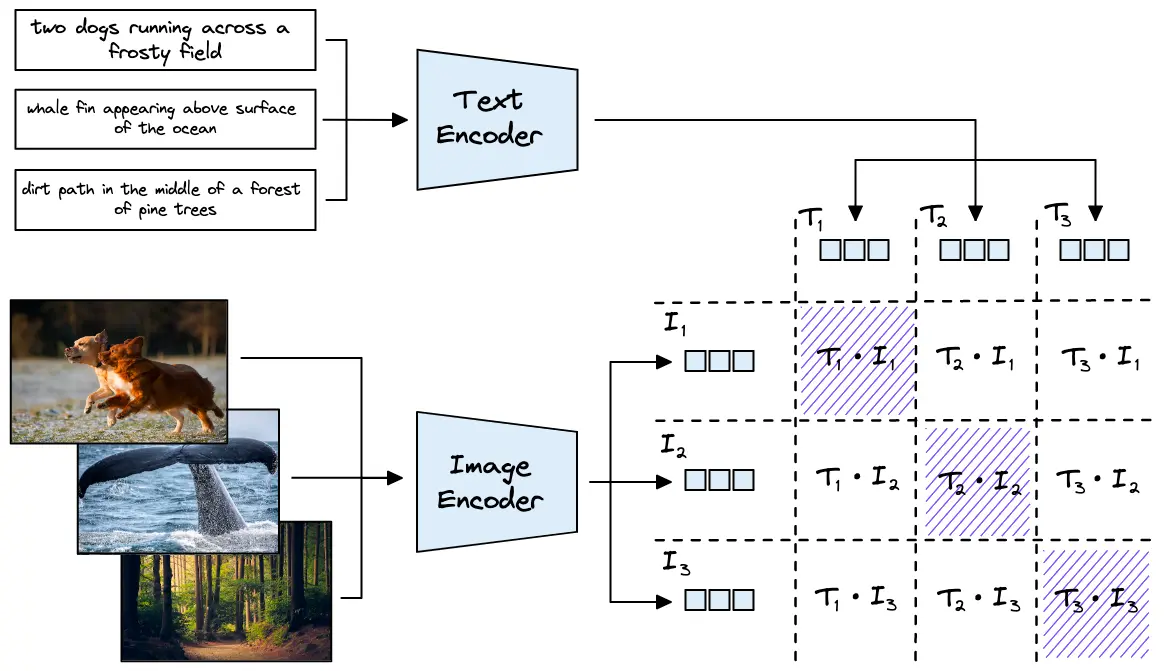
\includegraphics[width=1.0\textwidth]{images/clip_zero_shot_classification.png}
	\captionof{figure}{Minh họa quy trình phân loại zero-shot của CLIP. Embedding của ảnh được so sánh với các embedding của các prompt văn bản tương ứng với các lớp. Lớp có độ tương đồng cosine cao nhất sẽ được chọn.}
	\label{fig:clip_zero_shot}
\end{center}
% Keyword gợi ý: clip zero shot classification, contrastive language image pretraining

\subsection{Few-Shot Learning (FSL): Học cách Học}
\label{subsec:few_shot_learning}
\textbf{Mục tiêu:} Huấn luyện một mô hình có khả năng nhanh chóng học một khái niệm mới chỉ từ một vài ví dụ. Đây là một kịch bản cực kỳ phổ biến trong các ứng dụng thực tế, nơi dữ liệu cho các lớp mới thường rất khan hiếm.

\subsubsection{Các Phương pháp FSL}
\label{subsubsec:fsl_methods}
\begin{description}
	\item[Học Đo lường (Metric-based Learning):] Hướng tiếp cận này tập trung vào việc học một không gian nhúng tốt. Một khi đã có không gian này, việc phân loại một mẫu mới chỉ đơn giản là so sánh nó với các mẫu hỗ trợ (support set) đã biết. \textbf{Prototypical Networks} \cite{Snell2017} là một ví dụ điển hình: nó tính toán một "nguyên mẫu" (prototype) cho mỗi lớp bằng cách lấy trung bình các embedding của các mẫu hỗ trợ, và sau đó phân loại một mẫu truy vấn bằng cách tìm xem nó gần với nguyên mẫu nào nhất.
	\item[Siêu học (Meta-Learning):] Triết lý của meta-learning là "học cách học" (learning to learn). Mô hình được huấn luyện trên một loạt các "tác vụ" học tập nhỏ, mỗi tác vụ mô phỏng một kịch bản few-shot. Bằng cách tối ưu hóa hiệu năng trên nhiều tác vụ này, mô hình học được một bộ trọng số khởi tạo tốt hoặc một quy tắc cập nhật hiệu quả, cho phép nó thích nghi nhanh chóng với các tác vụ mới và chưa từng thấy. \textbf{MAML (Model-Agnostic Meta-Learning)} là một thuật toán meta-learning kinh điển.
	\item[Học chuyển giao và Tinh chỉnh Hiệu quả (Transfer Learning \& Parameter-Efficient Fine-Tuning):] Đây là cách tiếp cận thực tế và phổ biến nhất hiện nay.
	\begin{enumerate}
		\item Bắt đầu với một mô hình nền tảng (foundation model) mạnh mẽ đã được huấn luyện trước (ví dụ: ViT, CLIP, DINOv2).
		\item Thay vì tinh chỉnh (fine-tune) toàn bộ hàng trăm triệu tham số của mô hình (điều này sẽ gây ra overfitting nghiêm trọng với ít dữ liệu), chúng ta chỉ tinh chỉnh một phần rất nhỏ của mạng.
		\item Các kỹ thuật như \textbf{Adapter Tuning} (chèn các module nhỏ vào giữa các lớp), \textbf{LoRA (Low-Rank Adaptation)}, hay \textbf{Prompt Tuning} cho phép mô hình thích ứng với tác vụ mới chỉ bằng cách học thêm vài nghìn hoặc vài triệu tham số, trong khi giữ nguyên phần lớn xương sống của mô hình.
	\end{enumerate}
\end{description}

\subsection{Prompting Vision Models: Tương tác thay vì Huấn luyện lại}
\label{subsec:prompting_vision_models}
Sự ra đời của các mô hình ngôn ngữ lớn như GPT-3 đã phổ biến hóa khái niệm \textbf{"prompting"}—điều khiển hành vi của một mô hình khổng lồ chỉ bằng cách thay đổi câu lệnh đầu vào, thay vì phải huấn luyện lại nó. Ý tưởng này đã nhanh chóng được áp dụng cho các mô hình thị giác.

\textbf{Visual Prompting} là nghệ thuật thiết kế các đầu vào (prompts) để hướng dẫn một mô hình thị giác nền tảng thực hiện một tác vụ cụ thể.
\begin{description}
	\item[Text Prompting:] Như đã thấy với CLIP, đây là hình thức phổ biến nhất. Việc thiết kế các prompt văn bản tốt (ví dụ: sử dụng các template như "a photo of a {}" hoặc "an image of a {} in the wild") có thể cải thiện đáng kể hiệu năng zero-shot.
	\item[Visual Prompting:] Thay vì văn bản, prompt có thể là các tín hiệu thị giác.
	\begin{itemize}
		\item \textbf{Point/Box Prompts:} Trong các mô hình như \textbf{Segment Anything Model (SAM)}, người dùng có thể "prompt" mô hình bằng cách nhấp vào một điểm hoặc vẽ một chiếc hộp xung quanh một đối tượng để yêu cầu mô hình phân đoạn nó.
		\item \textbf{Learnable Visual Prompts:} Thêm một vài pixel hoặc một "patch" có thể học được vào ảnh đầu vào. Trong quá trình fine-tuning, chỉ các pixel của prompt này được cập nhật, trong khi backbone của mô hình vẫn được giữ nguyên.
	\end{itemize}
\end{description}

\begin{mdframed}[style=infobox]
	\textbf{Tương lai là "Promptable" AI}
	
	Xu hướng hiện tại đang hướng tới việc xây dựng các mô hình nền tảng đa năng, có thể được "điều khiển" bằng prompt để giải quyết nhiều tác vụ. Một mô hình duy nhất như SAM có thể thực hiện phân đoạn, một mô hình như Grounding DINO có thể thực hiện phát hiện vật thể dựa trên prompt văn bản. Điều này làm giảm đáng kể nhu cầu xây dựng các mô hình chuyên biệt cho từng tác vụ, mở ra một kỷ nguyên của AI linh hoạt và dễ tiếp cận hơn.
\end{mdframed}

\subsection{Kết luận: Hướng tới AI Tổng quát}
\label{subsec:zsl_fsl_conclusion}
Zero-shot Learning, Few-shot Learning, và Prompting không chỉ là những kỹ thuật riêng lẻ; chúng là những biểu hiện của một xu hướng lớn hơn hướng tới các hệ thống AI tổng quát và linh hoạt hơn. Chúng đã thay đổi căn bản cách chúng ta tương tác và triển khai các mô hình thị giác:
\begin{itemize}
	\item Chúng giảm đáng kể sự phụ thuộc vào dữ liệu gán nhãn thủ công, cho phép AI được áp dụng cho các bài toán "đuôi dài" (long-tail problems) với vô số các lớp hiếm.
	\item Chúng cho phép các mô hình thích ứng nhanh chóng với các miền và tác vụ mới, một khả năng cực kỳ quan trọng trong thế giới thực luôn thay đổi.
	\item Chúng là công nghệ nền tảng cho các hệ thống \textbf{AI đa phương thức, có khả năng lý luận}, có thể hiểu và tương tác với thế giới thông qua nhiều kênh thông tin khác nhau.
\end{itemize}
Trong kỷ nguyên của các mô hình nền tảng, câu nói "Một prompt tốt có thể giá trị hơn một quá trình huấn luyện lại" ngày càng trở nên đúng đắn. Việc hiểu và làm chủ các kỹ thuật này là chìa khóa để khai thác toàn bộ sức mạnh của thế hệ AI thị giác tiếp theo.

\section*{Tài liệu tham khảo}
\begin{itemize}
	\item[1] Radford, A., Kim, J. W., Hallacy, C., Ramesh, A., Goh, G., Agarwal, S., ... \& Sutskever, I. (2021). Learning transferable visual models from natural language supervision. In \textit{International Conference on Machine Learning (ICML)}. (Paper gốc về CLIP, nền tảng cho ZSL hiện đại).
	\item[2] Snell, J., Swersky, K., \& Zemel, R. (2017). Prototypical networks for few-shot learning. In \textit{Advances in neural information processing systems (NeurIPS)}. (Giới thiệu Prototypical Networks, một phương pháp FSL dựa trên metric-learning kinh điển).
	\item[3] Finn, C., Abbeel, P., \& Levine, S. (2017). Model-agnostic meta-learning for fast adaptation of deep networks. In \textit{International conference on machine learning (ICML)}. (Giới thiệu MAML, một thuật toán meta-learning có ảnh hưởng lớn).
	\item[4] Kirillov, A., Mintun, E., Ravi, N., Tou, H., Caron, M., ... \& Girshick, R. (2023). Segment anything. \textit{arXiv preprint arXiv:2304.02643}. (Một ví dụ về mô hình nền tảng có thể "prompt" bằng các tín hiệu thị giác).
	\item[5] Brown, T., Mann, B., Ryder, N., Subbiah, M., Kaplan, J. D., Dhariwal, P., ... \& Amodei, D. (2020). Language models are few-shot learners. In \textit{Advances in neural information processing systems (NeurIPS)}. (Paper về GPT-3, đã phổ biến hóa khái niệm prompting và in-context learning trong NLP).
	\item[6] Houlsby, N., Giurgiu, A., Jastrzebski, S., Morrone, B., De Laroussilhe, Q., ... \& Gelly, S. (2019). Parameter-efficient transfer learning for NLP. In \textit{International Conference on Machine Learning (ICML)}. (Giới thiệu Adapter Tuning, một kỹ thuật parameter-efficient fine-tuning).
\end{itemize}